\documentclass[presentation,professionalfonts]{beamer}


\usepackage[utf8]{inputenc}
\usepackage[T1]{fontenc}
\usepackage{graphicx}
\usepackage[normalem]{ulem}
\usepackage{amsmath}
\usepackage{IEEEtrantools}
\usepackage{bm}
\usepackage{hyperref}
\tolerance=1000
%% \usepackage{algorithm}
\usepackage{algorithm2e}
\usepackage{algpseudocode}
\usepackage{tikz}
\usepackage{xspace}
\usepackage{booktabs}
\usepackage{listings}
\usepackage{appendixnumberbeamer}
\usepackage{textcomp}

\usepackage[
backend=biber,
style=numeric,
sortlocale=en_US,
url=false,
doi=true,
eprint=false,
giveninits=false,
maxbibnames=20,
maxnames=20,
maxcitenames=4
]{biblatex}
\addbibresource{templ.bib}

\usepackage{lmodern}
\usefonttheme[onlymath]{serif}

\setbeamercovered{highly dynamic}
\setbeamertemplate{caption}[numbered]
\setbeamertemplate{bibliography item}[text]
\usetheme{TUW}

\DeclareMathOperator*{\argmin}{\arg\!\min}
\DeclareMathOperator*{\argmax}{\arg\!\max}

\newcommand{\semname}{Scheduling Algorithms for Clusters, Distributed Systems, and Multi-core Nodes}
\newcommand{\semester}{SS 2018}

\institute[TU Wien]{Seminar ``\semname''\\\semester}
\titlegraphic{
\includegraphics[height=.7cm]{./logos/par-logo.pdf}\quad
\includegraphics[height=.7cm]{./logos/info-logo.pdf}}

% change this, of course
\date{\today}
\title[Scheduling Jobs with Max-Min Fairness]{Scheduling Jobs across Geo-Distributed Datacenters with Max-Min Fairness}
\author[Aleksandr Lisianoi]{Aleksandr Lisianoi}

\begin{document}

\maketitle

\begin{frame}{Seminar Talk's Main Sources}
  \begin{enumerate}
  \item \fullcite{Chen2017}
  \end{enumerate}
\end{frame}

\AtBeginSection[]
{
 \begin{frame}<beamer>
 \frametitle{Plan}
 \tableofcontents[currentsection]
 \end{frame}
}

%% \begin{frame}{Outline}
%%   % \tableofcontents[currentsection]
%%   \tableofcontents
%% \end{frame}

\section{Introduction}
\begin{frame}{Scheduling Problem}
  \begin{center}
  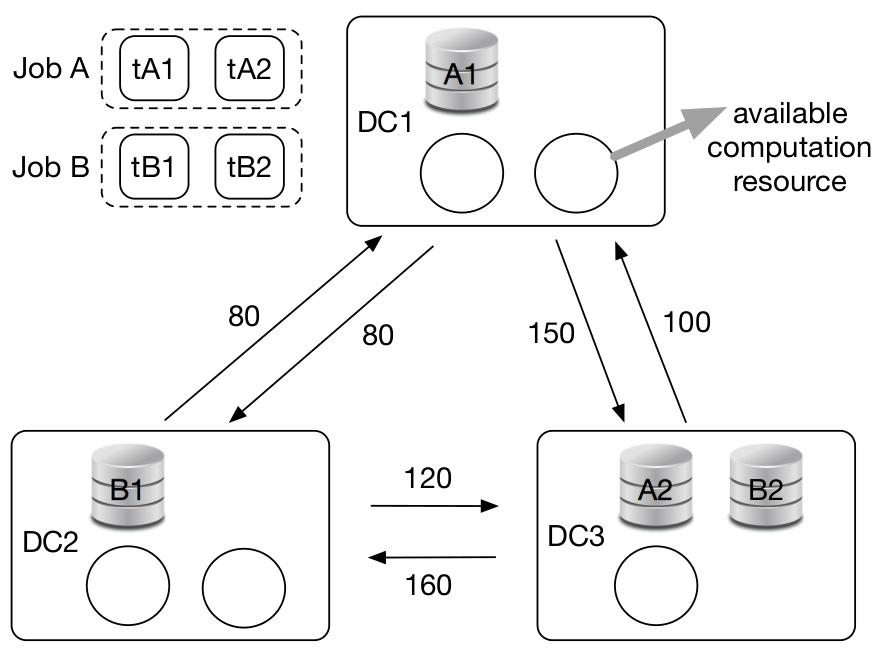
\includegraphics[width=0.8\textwidth]{fig1}\\
  image source: \textcite{Chen2017}
  \end{center}
\end{frame}

\begin{frame}{Main Topic}
  Running \emph{multiple} analytic jobs \emph{efficiently and fairly} when:
  \begin{itemize}
  \item each job requires a \emph{large amount of data} to run
  \item the data is stored in \emph{geographically distributed} datacenters
  \end{itemize}
\end{frame}

\begin{frame}{Important Factors}
  Geographic separation and a lot of data \textrightarrow{} \emph{network speed}
  \\~\\
  Multiple concurrent jobs \textrightarrow{} \emph{fair resource allocation}
\end{frame}

\begin{frame}{Main Contribution}
  A scheduling algorithm that in practice outperforms the default Apache Spark task scheduler under the following conditions:
  \begin{itemize}
  \item multiple concurrent jobs must be scheduled
  \item cluster workers are geographically separated
  \item external resource managers not present (e.g. YARN)
    \end{itemize}
\end{frame}

%% \begin{frame}{Typical Analytic Jobs}
%%   \begin{itemize}
%%   \item 2007 The New York Times: ~4 TiB, less than 24 hours for 1 job \\
%%     (\href{https://open.blogs.nytimes.com/2007/11/01/self-service-prorated-super-computing-fun/}{online article}, last access 21.04.2018)
%%   \item 2017 ALS at Spotify: ~100 PiB, ~2500 nodes, ~20k jobs per day \\
%%     (\href{https://labs.spotify.com/2017/10/16/big-data-processing-at-spotify-the-road-to-scio-part-1/}{online article}, last access 21.04.2018)
%%   \end{itemize}
%% \end{frame}

%% \begin{frame}{Fairness}
%%   \emph{Fairness}: all the participants get a fair share of the
%%   resources.
%%   \\~\\
%%   \emph{Max-Min fairness}: any attempt to increase any participant's
%%   share decreases some non-larger share of another participant.
%% \end{frame}

\section{Scheduling Algorithm}

\begin{frame}{Some Notation}
  \begin{IEEEeqnarray*}{llCl}
    \text{Datacenter: }                 & \mathcal{D}   &=& \left\{1, 2, \dots, J\right\} \\
    \text{Datacenter capacity: }        & \mathcal{A}   &=& \left\{a_1, a_2, \dots, a_J\right\} \\
    \text{Analytic job: }               & \mathcal{K}   &=& \left\{1, 2, \dots, K\right\} \\
    \text{Parallel tasks of a job: }    & \mathcal{T}_k &=& \left\{1, 2, \dots, n_k\right\} \\
    \text{Execution time of a task: }                 & e^k_{i, j} \\
    \text{Network transfer time of a task: } & c^k_{i, j}
  \end{IEEEeqnarray*}
\end{frame}

\newcommand{\flvr}{\langle\bm{v}\rangle}
\newcommand{\fbma}{\bm{\alpha}}
\newcommand{\flar}{\langle\fbma\rangle}
\newcommand{\fbmb}{\bm{\beta}}
\newcommand{\flbr}{\langle\fbmb\rangle}

\begin{frame}{Lexicographic Minimization}
  \begin{definition}[Non-increasingly sorted \(\langle\bm{v}\rangle\)]
    Let \(\flvr_k\) denote the \(k\)-th (\(1\leq k \leq K\)) largest element of \(\bm{v}\in\mathbb{Z}^K\), implying \(\flvr_1\geq\flvr_2\dots\geq\flvr_K\). Then \(\bm{\flvr} = \left(\flvr_1, \flvr_2, \dots, \flvr_K\right)\) represents the non-increasingly sorted version of \(\bm{v}\).
  \end{definition}
  \begin{definition}[Lexicographically smaller vector]
    For any \(\fbma\in\mathbb{Z}^K, \fbmb\in\mathbb{Z}^K\), if \(\flar_1\leq\flbr_1\) or \(\exists k\in \left\{1,2,\dots, K\right\}\) s.t. \(\flar_k\leq\flbr_k\) and \(\flar_i = \flbr_i, \forall i\in [1, \dots, k)\), then \(\fbma\) is lexicographically smaller than \(\fbmb\), denoted \(\fbma \preceq \fbmb\).
  \end{definition}
  \begin{definition}[Lexicographic minimization]
    Lexicographic minimization of vector \(\bm{f}\) is represented with \(\text{lexmin}_{\bm{x}}\bm{f}\) with the optimal solution \(\bm{x^*}\in\mathbb{R}^K\) s.t. \(\forall \bm{x}\in\mathbb{R}^K: \bm{f}(\bm{x^*})\preceq\bm{f}(\bm{x})\)
    \end{definition}
  \end{frame}

\newcommand{\foralltdk}{\forall i \in \mathcal{T}_k, \forall j\in\mathcal{D}, \forall k\in\mathcal{K}}
\newcommand{\fcapacity}{\sum_{k\in\mathcal{K}}\sum_{i\in\mathcal{T}_k} x^k_{i, j} \leq a_j}
\newcommand{\fcapacityq}{\forall j\in\mathcal{D}}
\newcommand{\fpresence}{\sum_{j\in\mathcal{D}}x^k_{i, j} = 1}
\newcommand{\fpresenceq}{\forall i\in\mathcal{T}_k, \forall k\in\mathcal{K}}

\begin{frame}{Initial Optimization Problem}
  \begin{IEEEeqnarray}{lrCll}
    \text{lexmin}_{\bm{x}} & \bm{f} &=&\left(\tau_1, \tau_2, \dots, \tau_K\right) &\\
    \text{s.t.} & \tau_k &=& \max_{i\in\mathcal{T}_k, j\in\mathcal{D}} x^k_{i, j}\left(c^k_{i, j} + e^k_{i, j}\right), &\forall k\in\mathcal{K} \label{eq:goal}\\
    &&& \fcapacity,  &\fcapacityq\label{eq:capacity}\\
    &&& \fpresence,  &\fpresenceq\label{eq:presence}\\
    &&& x^k_{i, j} \in \left\{0, 1\right\}. &\foralltdk\label{eq:onehot}
  \end{IEEEeqnarray}

  Constraint \eqref{eq:goal}: a job requires as long as its longest task. \\
  Constraint \eqref{eq:capacity}: capacity of the datacenter is not exceeded. \\
  Constraint \eqref{eq:presence}: each task is assigned to exactly one datacenter. \\
\end{frame}

\begin{frame}{Tractable Class of Optimization Problems}
  If optimization problem fulfills the following requirements:
  \begin{itemize}
  \item separable convex objective function
  \item totally unimodular linear constraints
  \end{itemize}
  then apply \(\lambda\)-representation and compute solution, see \textcite{Meyer1976}.

  \pause
  \begin{definition}[Separable function]
    \begin{center}
      \(f(x_1, x_2, \dots, x_K) = \sum_{i=1}^K f_i(x_i)\)
    \end{center}
  \end{definition}
  \begin{definition}[Convex function]
    \(\forall x_1, x_2 \in\bm{X},\forall t\in[0, 1]: f(tx_1 + (1 - t)x_2)\leq tf(x_1) + (1 - t)f(x_2)\)
  \end{definition}
  \begin{definition}[Totally unimodular matrix]
    Matrix \(M\) is a \emph{totally unimodular matrix} if its
    every \emph{square submatrix} \(A\) has \(\det A\in \{-1, 0,
    1\}\)    
    \end{definition}
\end{frame}

\newcommand{\flambdas}{\lambda^{k, 0}_{i, j} + \lambda^{k, 1}_{i, j}}
\newcommand{\fsmember}{\flambdas M^{\left(c^k_{i, j} + e^k_{i, j}\right)}}
\newcommand{\rplus}{\mathbf{R}^{+}}

%% \begin{frame}{Final Optimization Subproblem}
%%   \begin{IEEEeqnarray*}{Cl}
%%     \min_{\bm{x}, \bm{\lambda}} & \quad \sum_{k\in\mathcal{K}}\sum_{i\in\mathcal{T}_k}\sum_{j\in\mathcal{D}} \left(\fsmember\right) \\
%%     \text{s.t.}  & \quad x^k_{i, j} = \lambda^{k, 1}_{i, j}, \foralltdk \\
%%                  & \quad \flambdas = 1, \foralltdk \\
%%                  & \quad x^k_{i, j}, \lambda^{k, 0}_{i, j}, \lambda^{k, 1}_{i, j} \in \rplus, \foralltdk \\
%%     & \quad \fcapacity, \fcapacityq \\
%%     & \quad \fpresence, \fpresenceq
%%   \end{IEEEeqnarray*}
%% \end{frame}

\begin{frame}{Proposed Scheduling Algorithm}
  \begin{algorithm}[H]
    \SetKwInOut{Input}{Input}
    \SetKwInOut{Output}{Output}
    \Input{Data distribution \(d^{k, s}_i\), inter-datacenter bandwidth \(b_{s, j}\), execution time \(e_{i, j}^k\), datacenter capacities \(a_j\)}
    \Output{Task assignment \(x_{i, j}^k\)}

    Initialize \(\mathcal{K}' = \mathcal{K}\); \\
    \While{\(\mathcal{K}' \neq \emptyset\)} {
      Solve the tractable LP problem, obtain assignment \(\bm{x}\); \\
      Find largest completion time: \(x_{i^*, j^*}^{k^*} = \argmax\limits_{x_{i, j}^k \in\bm{x}}\phi\left(x_{i, j}^k\right)\); \\
      Fix \(x_{i^*, j}^{k^*},\forall j\in\mathcal{D}\); Remove them from \(\bm{x}\); \\
      Reduce resource capacity of the corresponding datacenter; \\
      Set \(\phi\left(x^{k^*}_{i, j}\right) = x^{k^*}_{i, j}\left(c^{k^*}_{i^*, j^*} + e^{k^*}_{i^*, j^*}\right),\forall i\in \mathcal{T}_{k^*}, \forall j\in \mathcal{D}\); \\
      Remove \(k^*\) from \(\mathcal{K}'\)
    }
  \end{algorithm}
\end{frame}

\section{Experimental Evaluation}

\begin{frame}{Experiment Architecture: Apache Spark}
  \begin{center}
  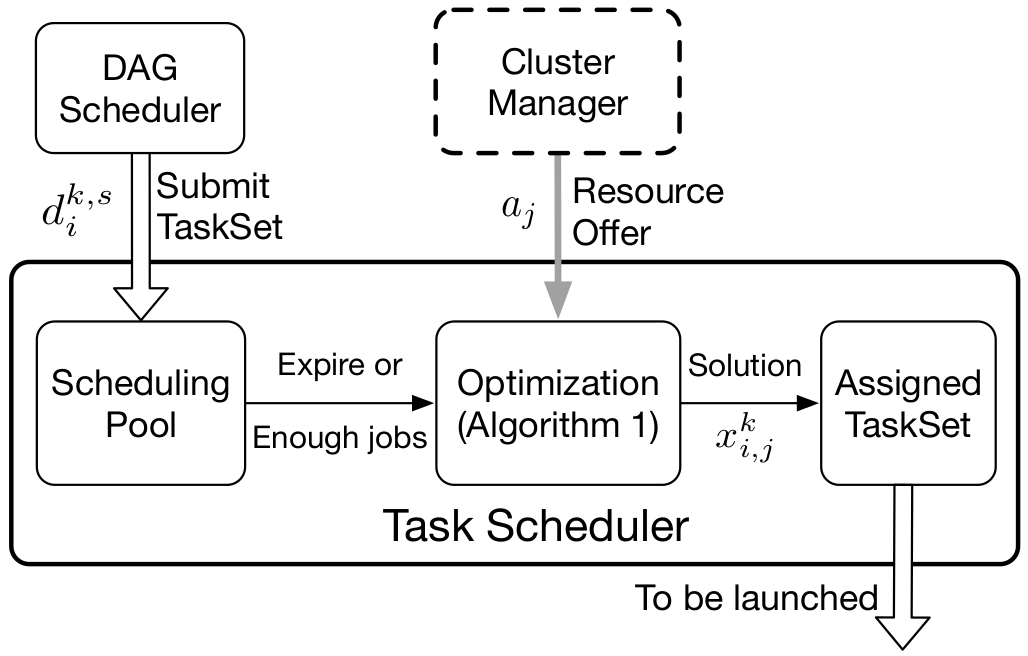
\includegraphics[width=\textwidth]{experiment_arch}\\
  image source: \textcite{Chen2017}
  \end{center}
  \end{frame}

\begin{frame}{Experiment Execution}
  \begin{itemize}
  \item Amazon EC2, 6 datacenters, 2 VMs of type \texttt{m3.large} each
  \item Ubuntu Server 14.04 LTS, Spark 1.6.1, Hadoop 2.6.4, Java 1.8, Scala 2.11.8
  \item Spark cluster in standalone mode, no external resource manager (e.g. YARN)
  \item Analytic job is legacy \texttt{Sort}:
    \begin{itemize}
    \item 3 tasks in parallel
    \item 100 MiB of data per task
    \item all data in different datacenters
    \end{itemize}
  \end{itemize}
\end{frame}

\begin{frame}
  \frametitle{Experimental Results}
  \begin{center}
  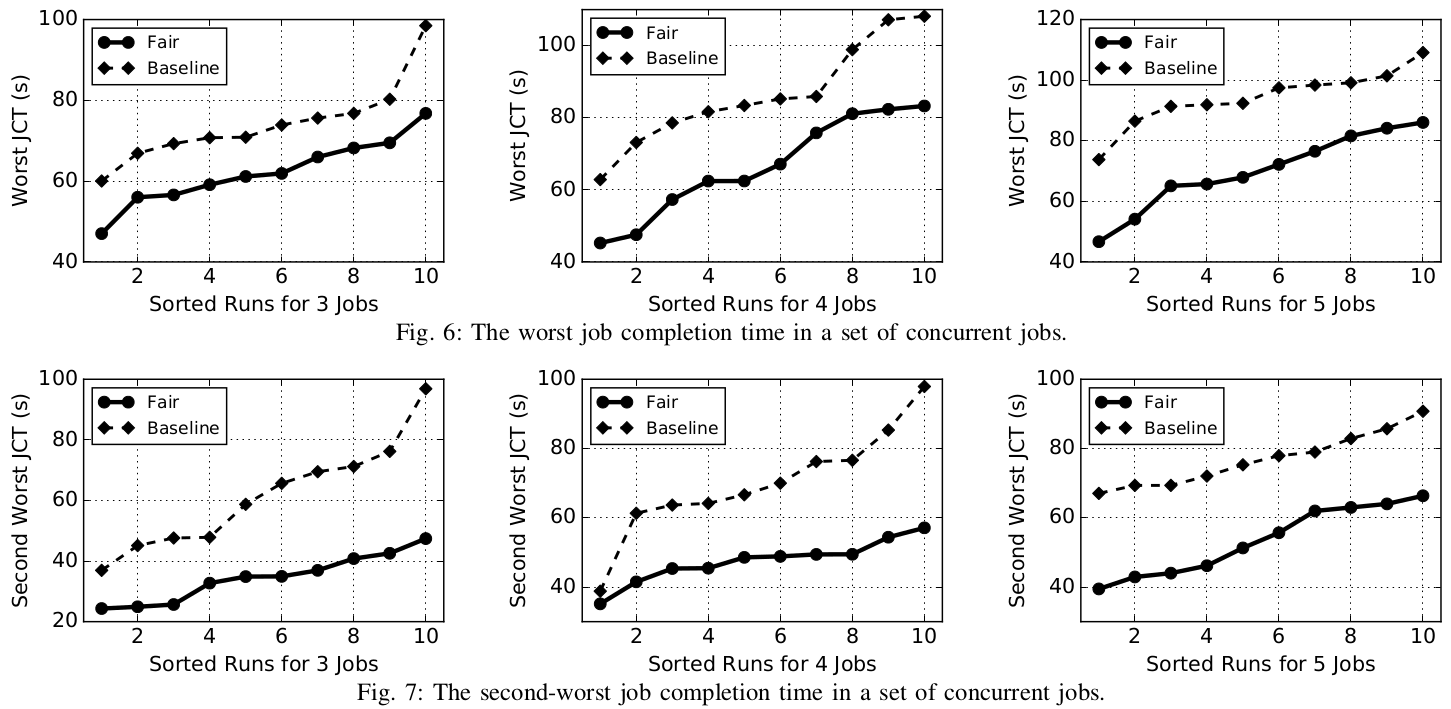
\includegraphics[width=1.03\textwidth]{main_result}\\
  image source: \textcite{Chen2017}
  \end{center}
\end{frame}

\begin{frame}{Time to Compute Assignments}
  \begin{center}
  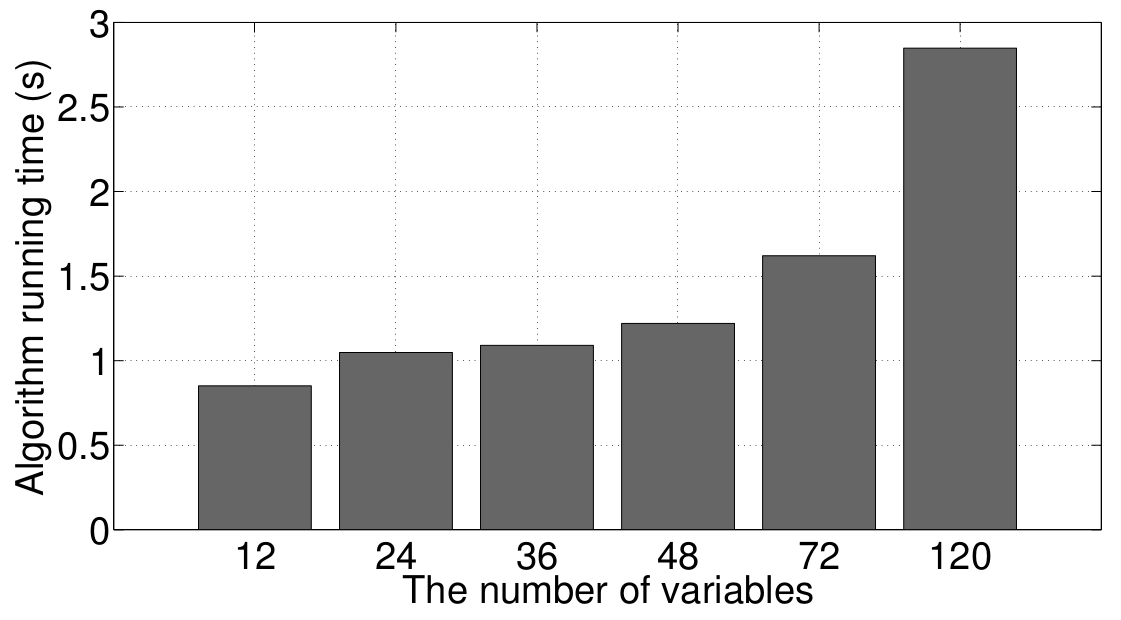
\includegraphics[width=1\textwidth]{algo_time}\\
  image source: \textcite{Chen2017}
  \end{center}
\end{frame}


\section{Conclusions}

\begin{frame}
  \frametitle{Conclusions}
  \begin{itemize}
  \item Outperformed default task scheduler of Apache Spark
  \item Nice transformation of an optimization problem
  \end{itemize}
\end{frame}


\begin{frame}[fragile]{References}
\printbibliography
\end{frame}

\appendix

\section{Matrix Definitions and Properties}

\begin{frame}{Unimodular Matrix}
  \begin{definition}[Unimodular Matrix]
    Matrix \(M\) is a \emph{unimodular matrix} if it is a \emph{square}, \emph{integer} matrix with \[\det M = \pm 1\]
  \end{definition}
  \begin{definition}[Unimodular Matrix]
    Matrix \(M\) is a \emph{unimodular matrix} if it is an
    \emph{integer}, \emph{invertible} matrix and its inverse is also
    an \emph{integer}, \emph{invertible} matrix.
  \end{definition}
  Examples: identity matrix, \emph{permutation matrix}, pascal matrix, \dots
\end{frame}

\begin{frame}{Totally Unimodular Matrix}
  \begin{definition}{Totally Unimodular Matrix}
    Matrix \(M\) is a \emph{totally unimodular matrix} if its every
    non-singular square submatrix is unimodular.
  \end{definition}

  \begin{definition}{Totally Unimodular Matrix}
    Matrix \(M\) is a \emph{totally unimodular matrix} if its every
    \emph{square submatrix} \(A\) has \(\det A\in \{-1, 0, 1\}\)
  \end{definition}

  \begin{definition}{Totally Unimodular Matrix}
    Matrix \(A\) is a \emph{totally unimodular matrix} if its every
    element \(A_{i, j}\in \{-1, 0, 1\}\) and any row subset \(R\) can
    be divided into two disjoint subsets \(R_1\) and \(R_2\) s.t.
    \[\left|\sum_{i\in R_1} a_{i, j} - \sum_{i\in R_2}a_{i, j}\right| \leq 1, \forall j\in{1, 2, \dots, n}\]
    \end{definition}
\end{frame}

\begin{frame}{Totally Unimodular Matrices in Optimization}
  Important well-known optimization fact: if \(M\) is totally
  unimodular and \(b\) is integral, then linear programs \(\left\{\min
  cx | Mx \geq b, x\geq 0\right\}\) and \(\{\max cx | Mx \leq b\}\)
  have integral optima for any \(c\).
\end{frame}

\section{Equivalent Transformation Overview}

\begin{frame}{Towards Single Objective and Linear Constraints}
  From multiple-objective to single-objective optimization:
  \begin{IEEEeqnarray}{ll}
    \min_{\bm{x}} & \quad \max_{k\in\mathcal{K}}\left(\tau_k\right) \\
    \text{s.t.}  & \quad \text{Constraints \eqref{eq:goal}, \eqref{eq:capacity}, \eqref{eq:presence} and \eqref{eq:onehot} hold}
  \end{IEEEeqnarray}

  \pause

  From non-linear constraints to linear constraints:

  \begin{IEEEeqnarray}{ll}
    \min_{\bm{x}} & \quad \max_{k\in\mathcal{K}}\left(\max_{i\in\mathcal{T}_k, j\in\mathcal{D}} x^k_{i, j}\left(c^k_{i, j} + e^k_{i, j}\right)\right) \\
    \text{s.t.}  & \quad \text{Constraints \eqref{eq:capacity}, \eqref{eq:presence} and \eqref{eq:onehot} hold}
  \end{IEEEeqnarray}

  \pause

  \begin{equation*}
        \text{Define: }\phi (x^k_{i, j}) = x^k_{i, j} (c^k_{i, j} + e^k_{i, j}), \forall i\in\mathcal{T}_k, j\in \mathcal{D}, k\in\mathcal{K}
  \end{equation*}

  \pause

  From minimizing the triple maximum to lexicographic minimization:
  \begin{IEEEeqnarray}{ll}
    \text{lexmin}_{\bm{x}} & \quad \bm{g} = \left(\phi(x^1_{1, 1}), \dots, \phi(x^k_{i, j}), \dots, \phi(x^K_{n_k, J})\right) \\
    \text{s.t.}           & \quad \text{Constraints \eqref{eq:capacity}, \eqref{eq:presence} and \eqref{eq:onehot} hold}
  \end{IEEEeqnarray}
\end{frame}

\begin{frame}{Towards a Separable Objective Function}
  \begin{IEEEeqnarray*}{lCl}
    \text{Define: }g^m &=& \text{element of vector }\bm{g}\text{ at position }m \\
    \text{Define: }M &=& |\bm{g}| = J\sum_{k = 1}^{K}n_k \\
    \text{Define: }\varphi(\bm{g}) &=& \sum_{m = 1}^{M}M^{g_m}
  \end{IEEEeqnarray*}
  \begin{lemma}
    \(\varphi(.)\) preserves the order of ``lexicographically no greater'' \(\preceq\), i.e.
    \[\bm{g}(x^*) \preceq \bm{g}(x) \iff \varphi(\bm{g}(x^*)) \leq\varphi(\bm{g}(x))\]
  \end{lemma}
\end{frame}

\begin{frame}{Transformation Plan Complete}
  \newcounter{x}\setcounter{x}{\value{equation}}\setcounter{equation}{5}
  \begin{IEEEeqnarray}{lrCll}
    \min_{\bm{x}} &&& \max_{k\in\mathcal{K}}\left(\tau_k\right) \\
    \setcounter{equation}{2}
    \text{s.t.} & \tau_k &=& \max_{i\in\mathcal{T}_k, j\in\mathcal{D}} x^k_{i, j}\left(c^k_{i, j} + e^k_{i, j}\right), &\forall k\in\mathcal{K} \\
    &&& \fcapacity,  &\fcapacityq \\
    &&& \fpresence,  &\fpresenceq \\
    &&& x^k_{i, j} \in \left\{0, 1\right\}. &\foralltdk
  \end{IEEEeqnarray}
  \setcounter{equation}{\value{x}}

  \begin{IEEEeqnarray}{ll}
    \min_{\bm{x}} & \quad \sum_{k\in\mathcal{K}}\sum_{i\in\mathcal{T}_k}\sum_{j\in\mathcal{D}} M^{\varphi(x^k_{i, j})} \\
    \text{s.t.}  & \quad \text{Constraints \eqref{eq:capacity}, \eqref{eq:presence} and \eqref{eq:onehot} hold}
  \end{IEEEeqnarray}
\end{frame}

\begin{frame}{Towards Removing Integrality Constraints}
  Lambda representation technique:
  \begin{IEEEeqnarray}{lCl}
    M^{\varphi\left(x^k_{i, j}\right)} &=& \sum_{s\in\{0,1\}} \lambda^{k, s}_{i, j}M^{s\left(c^k_{i, j} + e^k_{i, j}\right)} = \fsmember \IEEEeqnarraynumspace\\
    x^k_{i, j} &=& \sum_{s\in\{0, 1\}}s\lambda^{k, s}_{i, j} = \lambda^{k, 1}_{i, j} \\
    \sum_{s\in\{0, 1\}} \lambda^{k, s}_{i, j} &=& \flambdas = 1 \\
    \lambda^{k, s}_{i, j} &\in& \rplus
    \end{IEEEeqnarray}
\end{frame}

\begin{frame}{Integrality Constraints Removed}
  \begin{IEEEeqnarray}{Cl}
    \min_{\bm{x}, \bm{\lambda}} & \quad \sum_{k\in\mathcal{K}}\sum_{i\in\mathcal{T}_k}\sum_{j\in\mathcal{D}} \left(\fsmember\right) \\
    \text{s.t.}  & \quad x^k_{i, j} = \lambda^{k, 1}_{i, j}, \foralltdk \\
                 & \quad \flambdas = 1, \foralltdk \\
                 & \quad x^k_{i, j}, \lambda^{k, 0}_{i, j}, \lambda^{k, 1}_{i, j} \in \rplus, \foralltdk \\
    & \quad \fcapacity, \fcapacityq \\
    & \quad \fpresence, \fpresenceq
  \end{IEEEeqnarray}
\end{frame}

\begin{frame}{Back to Multiobjective Optimization}
  Subproblem produces \((k^*, i^*, j^*)\) with longest completion time
  \\~\\
  Set \(x^{k^*}_{i^*, j^*} = 1\) and \(x^{k^*}_{i^*, j} = 0, j\neq j^*\), remove from \(\bm{x}\)
  \\~\\
  Set completion times for \(x^{k^*}_{i, j}\), where \((i, j)\neq
  (i^*, j^*)\), to the worst completion time
  \end{frame}

\end{document}
